\chapter{Depth estimation and 3D reconstruction}
深度估计与三维重建(稠密重建)

\section{Depth estimation}
\subsection{Introduction}
\begin{figure}[H]
    \centering
    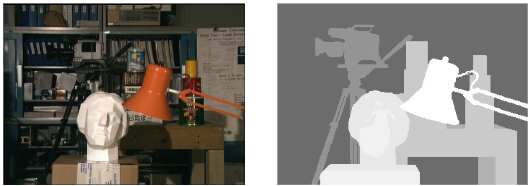
\includegraphics[width=0.68\textwidth]{Lec8/Compute depth maps}
    \caption{Compute depth maps}
\end{figure}

深度为离相机中心的距离, 注意是垂直距离还是直线距离(不同算法所给不同, 本节课是垂直距离). 

\subsubsection{Depth sensing}
\begin{enumerate}
    \item 避障
    \item 人脸识别(确保扫描的不是图像, 是三维的物体)
    \item 人机交互, 体感游戏
\end{enumerate}

\subsubsection{Active depth sensing}
主动式深度传感器
\begin{enumerate}
    \item LiDAR: Light Detection and Ranging (雷达, 测光反射的时间以测距离, ToF)
    \begin{enumerate}
        \item 昂贵
        \item 准确
        \item 最大可360\degree
    \end{enumerate}
    \item Structured light (结构光)
    \item Active stereo (主动式立体显像)
\end{enumerate}

\subsubsection{Passive depth sensing}
被动式深度感知
\begin{enumerate}
    \item Stereo (立体视觉)
    \item Monocular (单目估计, 依赖神经网络)
\end{enumerate}

\subsection{Stereo vision}
依靠双眼成像视差判断距离, 近的视差大, 远的视差小. 
\begin{figure}[H]
    \centering
    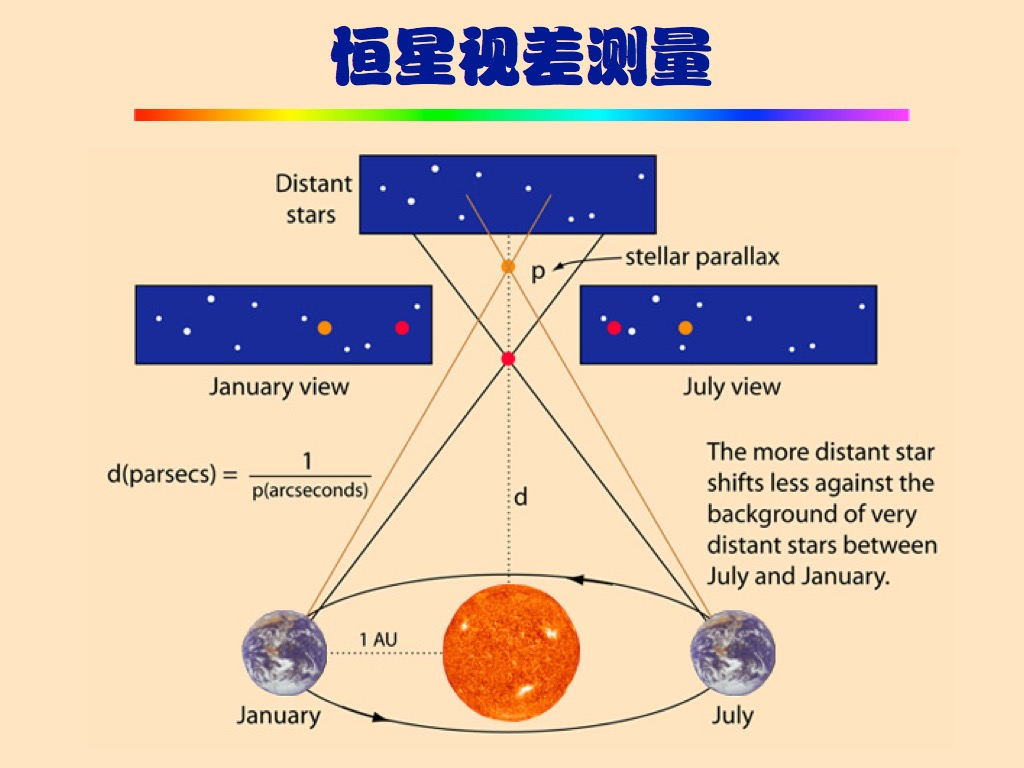
\includegraphics[width=0.08\textwidth]{Lec8/视差}
    \caption{视差}
\end{figure}

使用双目摄像机
\begin{enumerate}
    \item Find 2D-2D correspondences. 
    \item Triangulate. 
\end{enumerate}

问题是需要每个像素的匹配与相对高效的速率. 可使用光流解决, 但不够好, 因其并没有双目先验(点到点关系有极线约束). 

\begin{figure}[H]
    \centering
    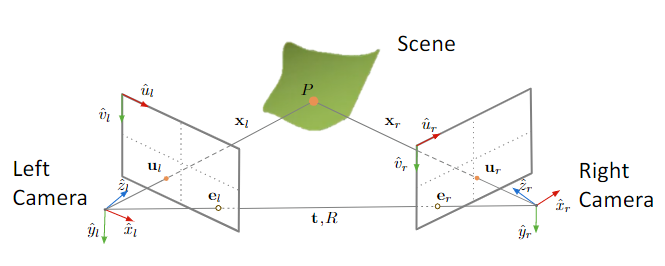
\includegraphics[width=0.68\textwidth]{Lec8/Epipolar geometry}
    \caption{Epipolar geometry}
\end{figure}

在这里使用了Epipolar Lines(极线). 

\begin{figure}[H]
    \centering
    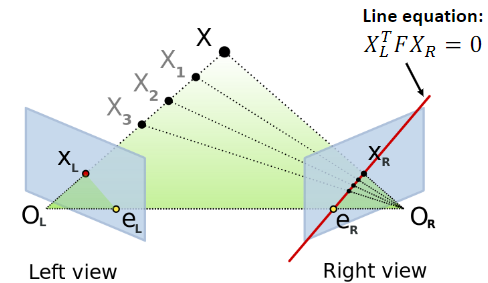
\includegraphics[width=0.68\textwidth]{Lec8/Epipolar line}
    \caption{Epipolar line}
\end{figure}

\begin{align*}
    X_L^T F X_R =0
\end{align*}

给定$X_L$, $X_R$必须满足这个方程. 这个方程就是上文的极线约束. 

\subsection{Basic stereo matching algorithm}

\subsubsection{For each pixel in the first image}

\begin{figure}[H]
    \centering
    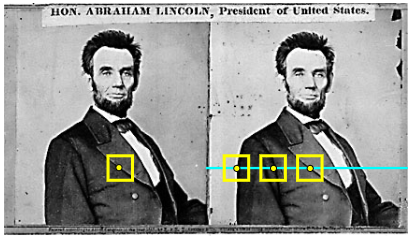
\includegraphics[width=0.68\textwidth]{Lec8/Basic stereo matching algorithm}
    \caption{Basic stereo matching algorithm}
\end{figure}

\begin{enumerate}
    \item Find corresponding epipolar line in the right image. 
    \item Search along epipolar line and pick the best match. 
\end{enumerate}

\subsubsection{Simplest case: Parallel images}

\begin{figure}[H]
    \centering
    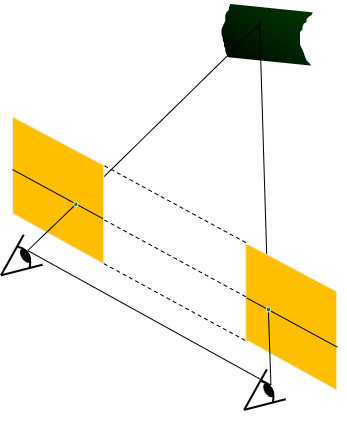
\includegraphics[width=0.38\textwidth]{Lec8/Parallel images}
    \caption{Parallel images}
\end{figure}

epipolarlines are horizontal scanlines. 
\begin{enumerate}
    \item Image planes of cameras are
    parallel to each other and to
    the baseline. 
    \item Camera centers are at same
    height. 
    \item Focal lengths are the same. 
    \item Then, epipolar lines fall along the horizontal scan lines of the images. 
\end{enumerate}

\subsubsection{Depth from disparity(视差)}

\begin{figure}[H]
    \centering
    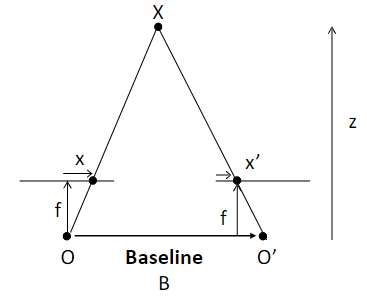
\includegraphics[width=0.38\textwidth]{Lec8/Disparity}
    \caption{Disparity}
\end{figure}

\begin{align*}
    \text{Disparity}=x-x'=\frac{B\cdot  f}{z}
\end{align*}

视差与深度严格成反比. 

\subsubsection{Stereo image rectification}

\begin{figure}[H]
    \centering
    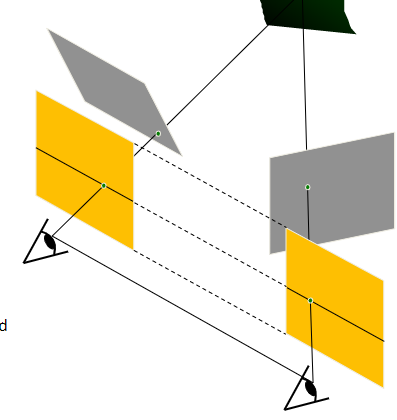
\includegraphics[width=0.28\textwidth]{Lec8/rectification}
    \caption{rectification}
\end{figure}

\begin{enumerate}
    \item Reproject image planes onto a common plane parallel to the line between camera centers. 
    \item Two homographies (3x3 transform), one for each input image reprojection. 
\end{enumerate}

\subsection{Stereo matching algorithms}

\subsubsection{Match pixels in conjugate epipolar lines}

\begin{enumerate}
    \item Assume brightness constancy. 
    \item This is a challenging problem. 
    \item Hundreds of approaches. 
\end{enumerate}

\subsubsection{Best match minimizes the dissimilarity}

\begin{figure}[H]
    \centering
    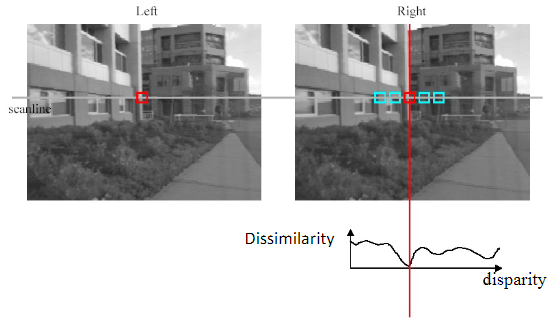
\includegraphics[width=0.48\textwidth]{Lec8/minimizes the dissimilarity}
    \caption{minimizes the dissimilarity}
\end{figure}

\subsubsection{Popular matching scores} 

\begin{enumerate}
    \item SSD (Sum of Squared Differences)
    \begin{align*}
        \sum_{x,y}\left| W_1(x,y)-W_2(x,y) \right|^2
    \end{align*}
    \item SAD (Sum of Absolute Differences)
    \begin{align*}
        \sum_{x,y}\left| W_1(x,y)-W_2(x,y) \right|
    \end{align*}
    \item ZNCC (Zero-mean Normalized Cross Correlation)
    \begin{align*}
        \frac{\sum_{x,y}(W_1(x,y)-\bar{W}_1)(W_2(x,y)-\bar{W}_2)}{\sigma_{W_1}\sigma_{W_2}} \,
        \text{where}\, \bar{W}_i=\frac{1}{n}\sum_{x,y}W_i, \, \sigma_{W_i}=\sqrt{\frac{1}{n}\sum_{x,y}(W_i-\bar{W}_i)^2}
    \end{align*}

    对亮度有不变性. 
\end{enumerate}

\subsubsection{Window size}
\begin{figure}[H]
    \centering
    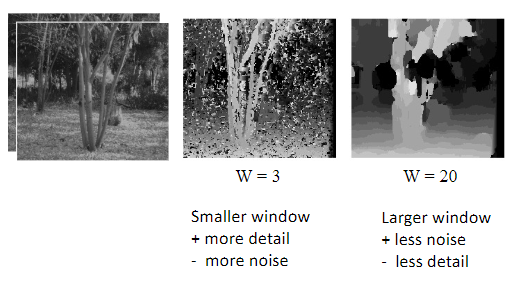
\includegraphics[width=0.58\textwidth]{Lec8/Window size}
    \caption{Window size}
\end{figure}

但即使是最佳 Window size 效果也不好, 但加图像分割(MRF, Markov 随机场)后效果显著. 

\begin{figure}[H]
    \centering
    \begin{subfigure}{0.28\textwidth}
        \centering
        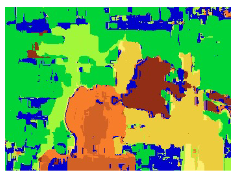
\includegraphics[width=\textwidth]{Lec8/best window size}
        \caption{best window size}
    \end{subfigure}
    \begin{subfigure}{0.28\textwidth}
        \centering
        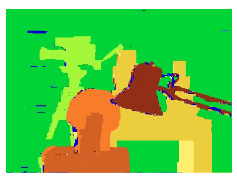
\includegraphics[width=\textwidth]{Lec8/Graph cuts-based method}
        \caption{Graph cuts-based method}
    \end{subfigure}
\end{figure}

\subsection{Stereo as energy minimization}
\begin{figure}[H]
    \centering
    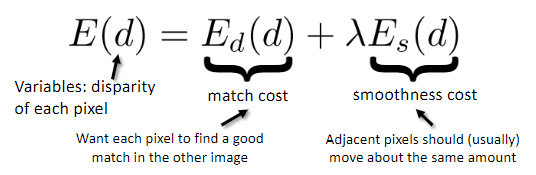
\includegraphics[width=0.48\textwidth]{Lec8/energy minimization}
    \caption{energy minimization}
\end{figure}

\begin{itemize}
    \item $E_d(d)=\sum_{(x,y)\in I}C\left(x,y,d(x,y)\right)$ eg: SSD, SAD, ZNCC(只跟每个像素各自深度有关系)
    \item $E_s(d)=\sum_{(p,q\in \varepsilon)}V(d_p,d_q)$(跟相邻像素深度有关系)
    \begin{itemize}
        \item $\varepsilon$: set of neighboring pixels.
        \item V
        \begin{itemize}
            \item $L_1$ distance: $V(d_p,d_q)=\left| d_p-d_q \right|$
            \item ``Potts model'': $V(d_p,d_q)=\left\{ \begin{array}{cc}
                0 & \text{if}\,d_p=d_q\\
                1 & \text{if}\,d_p\ne d_q
            \end{array} \right.$ (对边缘巨大差别不会过于光滑)
        \end{itemize}
    \end{itemize}
\end{itemize}

这是一个离散优化问题, 假设MRF($\varepsilon$)仅在一条线上, 可以用DP求解. 若MRF($\varepsilon$)是二维的随机场, 可以转化为最小割问题求解, 或使用机器学习的belief模型. 

\subsection{Stereo reconstruction pipeline}

\begin{enumerate}
    \item Calibrate cameras(相机标定)
    \item Rectify images(图像矫正)
    \item Compute disparity(计算视差)
    \item Estimate depth(估计深度)
\end{enumerate}

\subsubsection{Choosing the stereo baseline}
\begin{figure}[H]
    \centering
    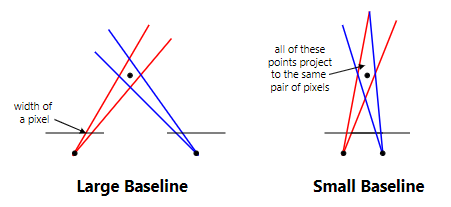
\includegraphics[width=0.38\textwidth]{Lec8/Baseline}
    \caption{Baseline}
\end{figure}
\begin{itemize}
    \item Too small: large depth error
    \item Too large: difficult search problem
\end{itemize}

\subsubsection{What will cause errors}
\begin{itemize}
    \item Camera calibration errors
    \item Poor image resolution
    \item Occlusions(遮挡)
    \item Violations of brightness constancy (specular reflections)
    \item Large motions
    \item Textureless regions(无纹理)
\end{itemize}

\subsection{Active stereo with structured light}
就像二维码, 给表面人为增加结构光, 使匹配更容易. 一般打的是红外的结构光(人眼不可见, 但可用红外相机), 甚至投影仪可以当作一个相机(投影的结构光已知). 

\begin{figure}[H]
    \centering
    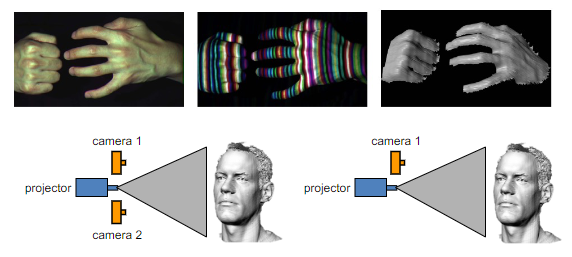
\includegraphics[width=0.38\textwidth]{Lec8/structured light}
    \caption{structured light}
\end{figure}

\subsection{Multi-view stereo}

Advantages: 
\begin{enumerate}
    \item Can match windows using more than 1 neighbor, giving \textbf{a stronger constraint}.
    \item If you have lots of potential neighbors, can \textbf{choose the best subset} of neighbors to match per reference image.
    \item Can reconstruct a depth map for each reference frame, and the merge into a \textbf{complete 3D model}.
\end{enumerate}

\subsubsection{Basic idea}

\begin{figure}[H]
    \centering
    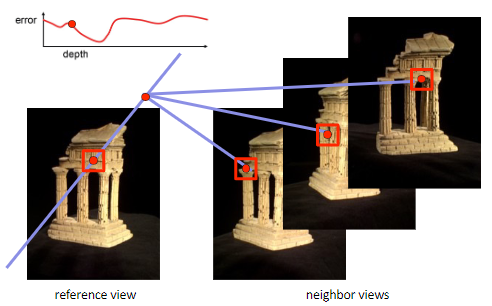
\includegraphics[width=0.38\textwidth]{Lec8/Multi-view stereo}
    \caption{Multi-view stereo}
\end{figure}

Compute the error for each depth value for each point in the reference image. Find the depth value that gives the smallest error. 源图片某深度后投影到其他图片获得一个block, 用此block与源图片算ZNCC, 最小的ZNCC对应的即为正确的深度. 

\subsubsection{Plane-Sweep}

\begin{figure}[H]
    \centering
    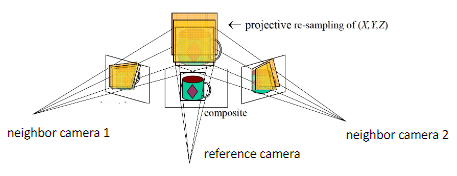
\includegraphics[width=0.38\textwidth]{Lec8/Plane-Sweep}
    \caption{Plane-Sweep}
\end{figure}

如何高效计算所有像素的 cost. 每个点所有深度的 cost 构成一个向量, 所有点的向量一起构成一个三维块, 每一个深度平面可以一起投影到图像(单应)可以得到 Cost Volumes(误差块), 用其可以得到深度信息. 效率没有显著提高(复杂度未变). 

\begin{figure}[H]
    \centering
    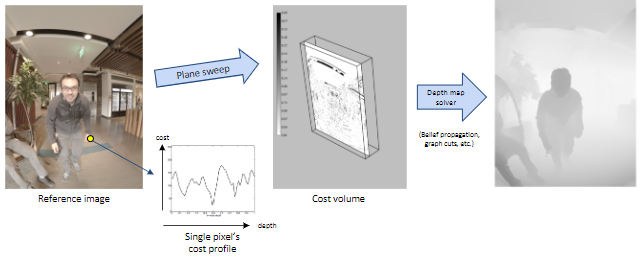
\includegraphics[width=0.38\textwidth]{Lec8/Cost Volumes}
    \caption{Cost Volumes}
\end{figure}

\subsubsection{PatchMatch}
图像块匹配. (一个随机化算法)

\begin{figure}[H]
    \centering
    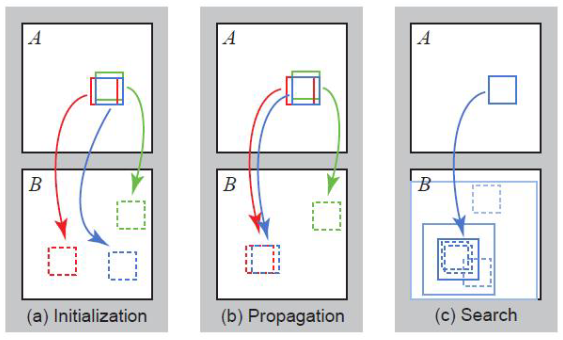
\includegraphics[width=0.58\textwidth]{Lec8/PatchMatch}
    \caption{PatchMatch}
\end{figure}

\begin{enumerate}
    \item Random initialization: Each pixel is given a random patch offset as initialization. (每个图像块随机进行匹配)
    \item Propagation(传播): Each pixels checks if the offsets from neighboring patches give a better matching patch. If so, adopt neighbor's patch offset. (相邻图像块的匹配是否更优, 如果优就更换匹配)
    \item Local search: (扰动以寻找更优的匹配)
    \begin{enumerate}
        \item Each pixels searches for better patch offsets within a concentric radius around the current offset.
        \item The search radius starts with the size of the image and is halved each time until it is 1.
    \end{enumerate}
    \item Go to Step 2 until converge.
\end{enumerate}

In MVS, replace patch offsets by depth values in the above algorithm. 

\section{3D reconstruction}

\subsection{3D Representations}

\begin{figure}[H]
    \centering
    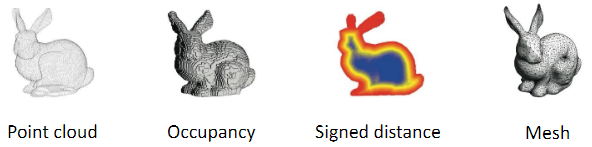
\includegraphics[width=0.58\textwidth]{Lec8/3D Representations}
    \caption{3D Representations}
\end{figure}

\begin{itemize}
    \item Point cloud (点云)
    \item Volume(体素, voxel) (非常占用空间)
    \begin{itemize}
        \item Occupancy (占用)
        \item Signed Distance Function(SDF) (点到物体表面的距离) 
        \item Truncated Signed Distance Function (TSDF) (截断距离场): Truncation SDF’s distance value to $[-1, 1]$ (太远的不记录具体值, 就为1了)
    \end{itemize}
    \item Mesh (网格): usually triangle mesh.  (甚至可以贴材质)
    
    Texture Mapping(纹理贴图): 每个网格顶点给一个坐标(O-uv), 以此绘制二维纹理图. 

    \begin{figure}[H]
        \centering
        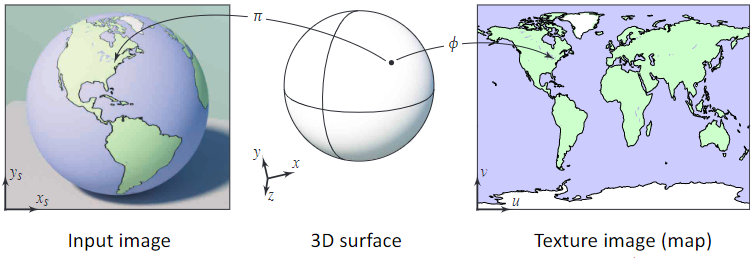
\includegraphics[width=0.68\textwidth]{Lec8/Texture Mapping}
        \caption{Texture Mapping}
    \end{figure}
    
\end{itemize}

三维重建就是为了获得Mesh与对应的纹理图. 

\subsection{3D surface reconstruction}
Fuse depth maps into a complete 3D mesh. (将多张深度图融合成为三维网格)

\begin{enumerate}
    \item Depth maps $\longrightarrow$ TSDF/occupancy volume (深度图到体素)
    \begin{enumerate}
        \item Kinest Fusion
        \item Poisson reconstruction $\star$
    \end{enumerate}
    \item TSDF/occupancy volume $\longrightarrow$ mesh (体素到网格)
\end{enumerate}

为何从点云到体素再到网格? 
\begin{enumerate}
    \item 操作简单
    \item 去噪简单 (在体素上去噪)
\end{enumerate}

\subsubsection{Poisson reconstruction}
将深度图转化为体素. 
\begin{enumerate}
    \item 将深度图化为点云. (从二维到三维的反投影)
    \begin{align*}
        \left\{ \begin{array}{l}
            z=depth(i,j)\\
            x=\frac{(j-e_x)\times z}{f_x}\\
            y=\frac{(i-e_y)\times z}{f_y}\\
        \end{array} \right.
    \end{align*}

    \item 计算每个点的法向量(normal vector): 取周围一些点拟合平面计算法向量 or 进行三维的主成分分析, 取最小的主成分. 
    \item 将点转化为体素

    \begin{figure}[H]
        \centering
        \begin{subfigure}{0.48\textwidth}
            \centering
            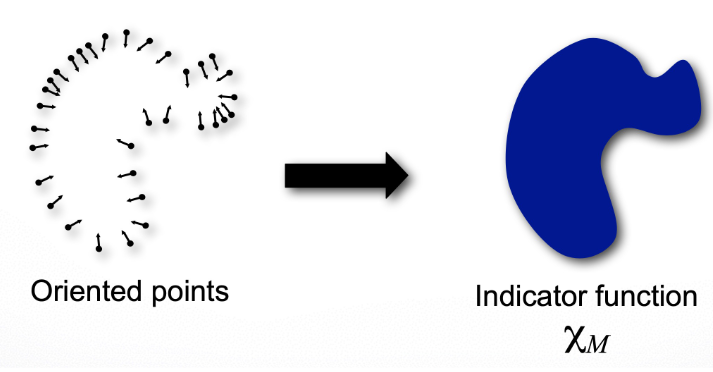
\includegraphics[width=\textwidth]{Lec8/Represent surface}
        \end{subfigure}
        \begin{subfigure}{0.48\textwidth}
            \centering
            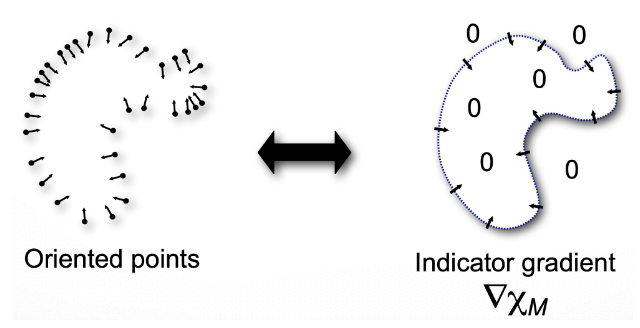
\includegraphics[width=\textwidth]{Lec8/Gradient Relationship}
        \end{subfigure}
        \caption{Represent surface}
    \end{figure}
    
    \begin{align*}
        \chi_{M}(p)=\left\{\begin{array}{ll}
            1 & \text { if } p \in M \\
            0 & \text { if } p \notin M
        \end{array}\right.
    \end{align*}

    \begin{enumerate}
        \item Represent the oriented points by a vector field $\vec{V}$
        \item Find the function $\chi$ whose gradient best approximates $\vec{V}$ by minimizing: 
        \begin{align*}
            \min_{\chi} \left\| \nabla \chi -\vec{V} \right\|
        \end{align*}
        \item Applying the divergence operator, we can transform this into a Poisson problem: (使用泊松方程求解)
        \begin{align*}
            \nabla \times (\nabla \chi) = \nabla \times \vec{V} \Longleftrightarrow \Delta \chi =\nabla \times \vec{V}
        \end{align*}
    \end{enumerate}
    
\end{enumerate}

\subsubsection{Marching cubes}
从体素提取网格. 

\begin{figure}[H]
    \centering
    \begin{subfigure}{0.28\textwidth}
        \centering
        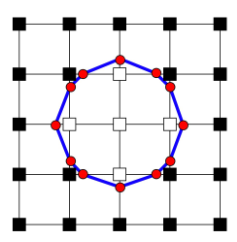
\includegraphics[width=\textwidth]{Lec8/Marching Squares (2D)}
        \caption{Marching Squares (2D)}
    \end{subfigure}
    \begin{subfigure}{0.28\textwidth}
        \centering
        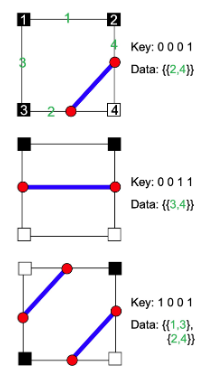
\includegraphics[width=0.58\textwidth]{Lec8/Connect vertices by lines}
        \caption{look-up table}
    \end{subfigure}
    \caption{Marching Squares (2D)}
\end{figure}

For each grid cell with a sign change
\begin{enumerate}
    \item Create one vertex on each grid edge with a sign change.
    \item Connect vertices by lines.
    \begin{enumerate}
        \item Lines should not intersect
        \item Use a pre-computed look-up table
    \end{enumerate}
    \item Location of the vertex can be determined by linear interpolation of SDF values.
\end{enumerate}

\begin{figure}[H]
    \centering
    \begin{subfigure}{0.28\textwidth}
        \centering
        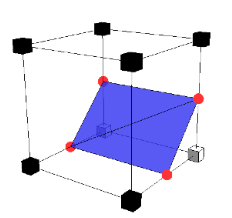
\includegraphics[width=\textwidth]{Lec8/Marching Cubes (3D)}
        \caption{Marching Squares (3D)}
    \end{subfigure}
    \begin{subfigure}{0.28\textwidth}
        \centering
        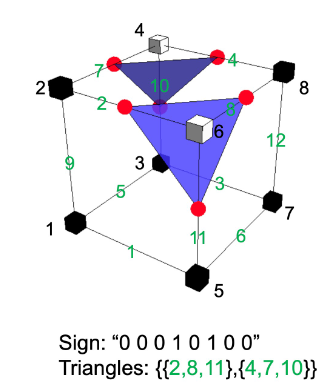
\includegraphics[width=0.38\textwidth]{Lec8/Connect vertices by triangles}
        \caption{look-up table}
    \end{subfigure}
    \caption{Marching Squares (3D)}
\end{figure}

For each grid cell with a sign change


\begin{enumerate}
    \item Create one vertex on each grid edge with a sign change
    \item Connect vertices by triangles
    \begin{enumerate}
        \item Triangles should not intersect
        \item Much more complicated than 2D cases
        \item But it still has look-up table
        \begin{itemize}
            \item $2^8=256$ sign configurations
            \item 15 configurations in total (considering symmetry)
        \end{itemize}
    \end{enumerate}
\end{enumerate}